\subsection{Principal Component Analysis}

Principal component analysis is a dimensionality reduction technique that transforms high-dimensional correlated data into a smaller set of uncorrelated variables.
The algorithms task is to handle the high dimensional vector spaces generated by time delay embeddings. Rather than operating on the raw multi variable data directly, principal component analysis takes the d-dimensional embedding vectors into an orthogonal coordinate system. The method identifies the directions of maximum variance (the principle components), thereby compressing the high dimensional space trajectories into a lower-dimensional subspace, most commonly two dimensions, while preserving the dominant dynamic characteristics of the vibration signal.
\label{section:foundation}
\subsection{Foundation}
Plotting the raw TDE output yields a point cloud with a complex geometry in $d$-dimensional space. This point cloud is characterized by two main properties: directions of maximum variance and their corresponding magnitudes. The directions give the orientation in space where the data varies, and the magnitudes tell how much the data spreads in each direction. The directions where the data varies the most are exactly where the information lies; on the other hand, noise can be found where very little variation is present.
\begin{figure}[H]
\centering
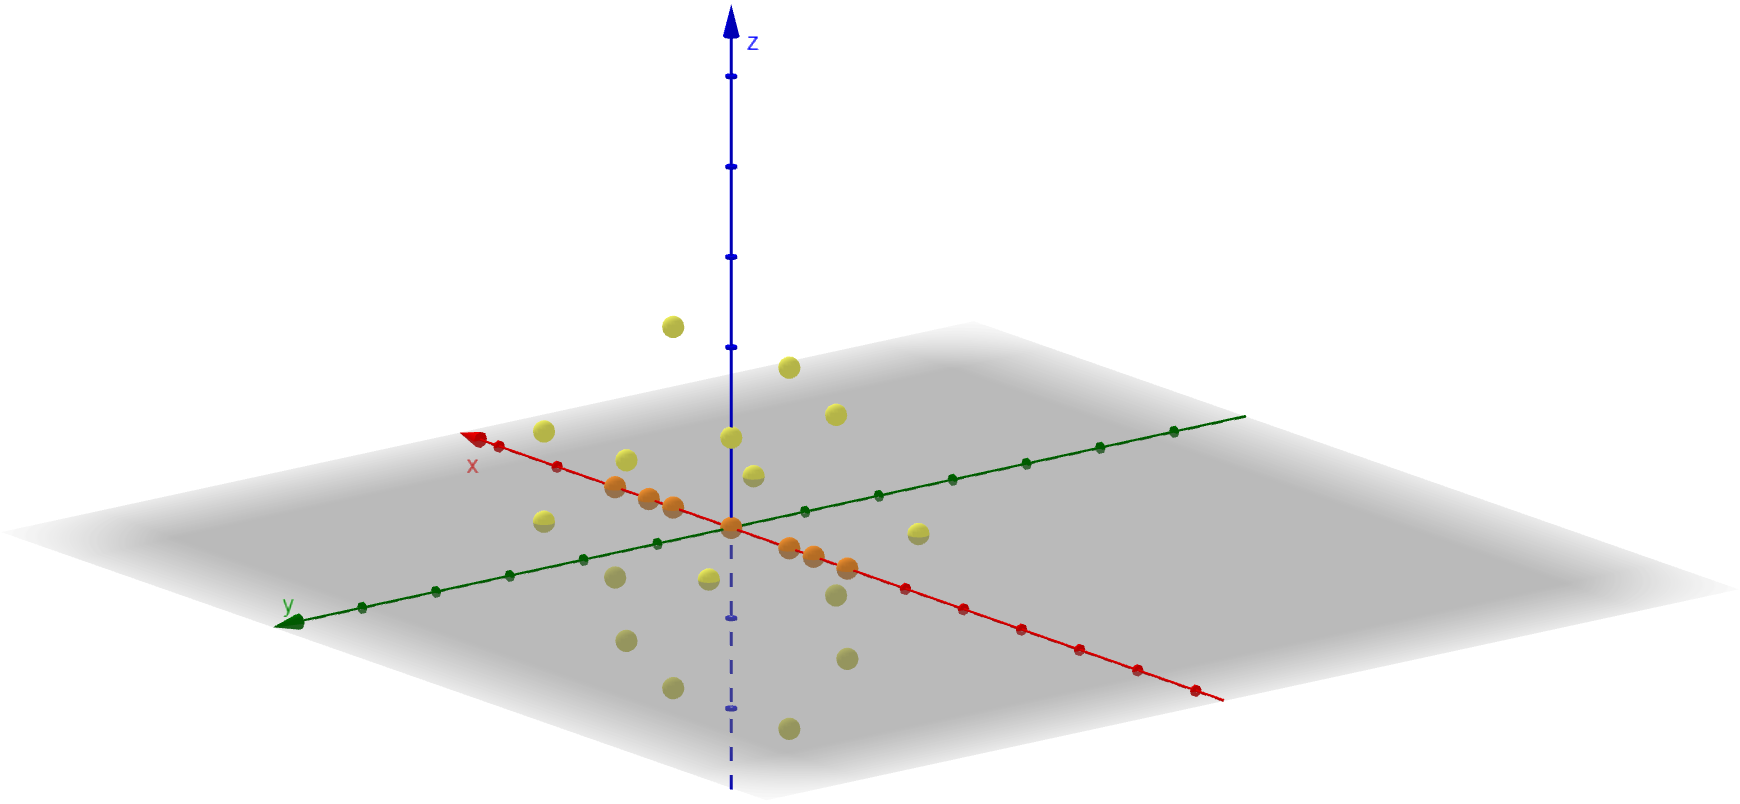
\includegraphics[width=0.7\textwidth]{figures/3dPointcloud.png}
\caption{Visualization of a 3D phase-space point cloud (yellow) and its 1D projection along the principal axis of maximum variance (orange).}
\label{fig:pointCloud}
\end{figure}
One possible approach would be to project all these points onto one single dimension. However, as visualized in Figure~\ref{fig:pointCloud}, when projecting all points onto a single axis, all additional data is lost(demonstrated by the orange points).
When a point $\mathbf{x}$ is projected onto a unit vector $\hat{\mathbf{u}}$, the resulting projected vector $\mathbf{x}'$ lies along $\hat{\mathbf{u}}$ with a magnitude defined by the inner product $\mathbf{x}^T \hat{\mathbf{u}}$:
\begin{equation}
\mathbf{x}' = (\mathbf{x}^T \hat{\mathbf{u}}) \hat{\mathbf{u}}
\end{equation}
The squared inner product $(\mathbf{x}^T \hat{\mathbf{u}})^2$ represents the magnitude of the projection. This squared quantity is minimized when $\mathbf{x}$ is orthogonal to $\hat{\mathbf{u}}$ and maximized when $\mathbf{x}$ is parallel to it. 

The method tries to find the unit vector $\hat{\mathbf{u}}$ that maximizes the sum of these squared projections across the entire dataset. Using the sample covariance matrix
\begin{equation}
\mathbf{C} = \frac{1}{N} \sum_{i=1}^{N} \mathbf{x}_i \mathbf{x}_i^T
\label{eq:covariance_matrix}
\end{equation}
the variance of the projected data is given by $\hat{\mathbf{u}}^T \mathbf{C} \hat{\mathbf{u}}$. Maximizing this variance subject to the constraint $\hat{\mathbf{u}}^T \hat{\mathbf{u}} = 1$ leads to the eigenvalue equation:
\begin{equation}
\mathbf{C}\hat{\mathbf{u}} = \lambda\hat{\mathbf{u}}
\label{eq:eigenvalue_equation}
\end{equation}
This proves that the principal directions of the data correspond to the eigenvectors of the covariance matrix $\mathbf{C}$. Since the variance along any given principal axis equals its corresponding eigenvalue $\lambda$, the eigenvector associated with the largest eigenvalue is the optimal direction that preserves the maximum amount of information.
\subsection{Computation}
Prior to computing the covariance matrix, the dataset has to be centered. This step is a mandatory preprocessing step in principal component analysis to ensure that the origin of the coordinate system matches with the sample mean $\boldsymbol{\mu}$. Without centering, the first principal component would reflect the shift of the dataset relative to the origin rather than displaying the directions of maximum variance. Here, the mean vector is defined by:
\begin{equation}
\boldsymbol{\mu} = \frac{1}{N} \sum_{i=1}^{N} \mathbf{x}_i
\label{eq:mean_vector}
\end{equation}
Following this, the centered vector $\tilde{\mathbf{x}}_i$ for each data point is defined as:
\begin{equation}
\tilde{\mathbf{x}}_i = \mathbf{x}_i - \boldsymbol{\mu}
\label{eq:centering_vector}
\end{equation}
Where $X$ is the current window mean. 
The covariance matrix $S$is then computed as:
\begin{equation}
\mathbf{S} = \frac{1}{n-1} \tilde{\mathbf{X}}^T \tilde{\mathbf{X}}
\end{equation}
The resulting covariance matrix $C$ quantifies how each pair of embedded variables varies together. By performing an eigen decomposition of the covariance matrix it gives back its eigenvalues $\lambda_1 ,\lambda_2....\lambda_d$ and corresponding eigenvectors $\mathbf{u}_1, \mathbf{u}_2, \dots, \mathbf{u}_d$, where each one of the eigenvalues $\lambda$ represents the variance captured along its its associated principal component\parencite[p.~382]{rencher2002methods}.
The resulting principal components scores represent the transformed data coordinates in the new orthogonal space are calculated by projecting the centered time delay embedding data matrix $\tilde{X}$ onto the matrix of eigenvectors $\mathbf{U} = [\mathbf{u}_1, \mathbf{u}_2, \dots, \mathbf{u}_d]$:
\begin{equation}
\mathbf{Z} = \tilde{\mathbf{X}}\mathbf{U}
\label{eq:pca_scores}
\end{equation}
Here, $\mathbf{Z} \in {R}^{N \times d}$ contains the projected principal component scores, where each column $i$ corresponds to the projection along the $i$-th eigenvector $\mathbf{u}_i$ where $\mathbf{U}$ denotes the matrix of extracted eigenvectors. For this specific area of application only the first two principal components $z_1$ and $z_2$ are kept. These components capture the most of the variance in the system while reducing the data from any $d$ down to two dimensions, which is easier to plot. Combining time delay embedding  with principal component analysis is especially effective in this use case because time delay embedding reconstructs the system dynamics in phase space, while principal component analysis is able to identify the lower-dimensional projection that preserves maximum variance, thereby making structural anomalies more visible. 
Only the first two principal components are kept as these components explain the major variance in the data. This allows a wide range of applications not only to anomaly detection but also to broader domain tasks requiring information preserving dimensionality reduction like image or data compression.


